% !TeX spellcheck = de_DE
\documentclass[12pt,a4paper]{article}
\usepackage[utf8]{inputenc}
\usepackage[german]{babel}
\usepackage[T1]{fontenc}
\usepackage{amsmath}
\usepackage{amsfonts}
\usepackage{amssymb}
\usepackage{graphicx}
\usepackage[left=2.5cm,right=2.5cm,top=2cm,bottom=2cm]{geometry}
\usepackage{float}

%\usepackage{subcaption}
\usepackage{subfig}
\usepackage{siunitx}
\usepackage{verbatim} 


\author{Gruppe B2 \\ Máté Farkas, Maria Spethmann}
\title{Protokoll Michelson-Interferometer \\ Physikalisches Grundpraktikum 2}


\begin{document}
	\maketitle
	\thispagestyle{empty} % Keine Seitenzahl auf der Titelseite
	\newpage
	\pagestyle{headings} % Seitenzahlen oben, Section und Subsection in Kopfzeile
	\tableofcontents
	\newpage


\section{Einleitung}
Bei diesem Versuch vermessen wir mithilfe eines Michelson-Interferometers die Wellenlänge eines unbekannten Lasers. Anschließend bestimmen wir die Druckabhängigkeit des Brechungsindexes von Luft.
\section{Physikalische Grundlagen} 
Bei einem Michelson-Interferometer interferiert Licht durch Amplitudenaufspaltung mit sich selbst und erzeugt ein Interferenzmuster, das R"uckschl"usse "uber beispielsweise Wellenl"ange oder Lichtgeschwindigkeiten gibt. Vorraussetzung f"ur Interferenz ist die Nutzung von koh"arentem Licht, also Wellenfronten, die eine "ortlich und zeitlich feste Phasenbeziehung zueinander haben. Laserstrahlen erf"ullen diese Bedingung.\\
Bei einem Michelson-Interferometer werden Laserstrahlen der Wellenl"ange $\lambda$ zun"achst an einem Strahlenteiler getrennt und auf verschiedene Bahnen geleitet. Die beiden Teilstrahlen werden nach unterschiedlichen Strecken jeweils gespiegelt und am selben Strahlteiler wieder zusammengef"uhrt. Die Strahlen "uberlagern sich nach dem Superpositionsprinzip, und weil sie unterschiedliche optische Wege mit Differenz $2d$ zurückgelegt haben, bildet sich ein Interferenzmuster. Abh"angig vom  "Offnungswinkel $\theta$ des Laserstrahls ergeben sich ringf"ormige Maxima, die sogenannten Interferenzringe:
\begin{equation}\label{eq:Interferenzmuster}
2d\cos(\theta)=m\lambda,\qquad m=0,1,2,...
\end{equation}
In diesem Versuch betrachten wir f"ur unsere Berechnungen nur das Hauptmaximum ($\theta=0$), sodass gilt
\begin{equation}\label{eq:Grundgleichung}
2d=m\lambda,\qquad m=0,1,2,...
\end{equation}
Die optische Wegl"ange einer Strecke $l$ errechnet sich durch 
\begin{equation}\label{eq:d=nl}
d=n\cdot l
\end{equation}
wobei der Brechungsindex $n=\frac{c}{v}$ das Verh"altnis zwischen Lichtgeschwindigkeit im Vakuum $c$ und im Medium $v$ angibt.
Der Brechungsindex ist druckabhängig und lässt sich in Luft bei einer Taylorentwicklung um $P=0$ in linearer Ordnung annähern durch 
\begin{equation}
n_{\text{Luft}}(P)=1+\frac{\Delta n}{\Delta P}\cdot P
\end{equation}
mit entsprechendem Koeffizienten  $\frac{\Delta n}{\Delta P}$, der in diesem Versuch bestimmt werden soll.

\section{Kalibrierung des Feinsteinstelltriebs}

\subsection{Versuchsaufbau}
Das in diesem Versuch verwendete Michelson-Interferometer besteht im Grundaufbau aus einem Laser, vier Spiegeln, einer Linse mit Brennweite +20mm, einem Strahlteiler und einem Schirm. Die Elemente sind wie in Abb.~\ref{Aufbau} mit Magnetf"u\ss en auf einer magnetischen Basisplatte angeordnet.  
Das Laserlicht wird über einen Spiegel (M1) durch eine Linse (L) gelenkt, die den Öffnungswinkel vergrößert, um mehrere Interferenzringe sichtbar zu machen. Anschließend fällt der Lichststrahl "uber einen weiteren Spiegel (M2) auf einen Strahlenteiler (ST). Dieser teilt den Strahl auf zwei senkrecht zueinander stehende Wege auf, an deren Ende je ein Spiegel (M3,M4) steht. Einer der Spiegel (M3) ist an einem Feinsteinstelltrieb mit Mikrometerschraube befestigt und l"asst sich somit manuell parallel zur Einfallsrichtung des Lichtes verschieben. Die Lichtstrahlen werden zur"uck zum Strahlenteiler reflektiert, wo jeweils ein Teil zurück zum Laser und eine anderer Teil auf dem Schirm (S) gelenkt wird. Am Schirm bildet sich ein Interferenzmuster gemäß Gl.~\eqref{eq:Interferenzmuster}.
Die Bauteile haben die richtige Position und Ausrichtung, wenn sich die Teilstrahlen ohne Hinzunahme der Linse genau am gleichen Ort auf dem Schirm und an der Austritts"offnung des Laserger"ats treffen. Zur genaueren Einstellung des Strahlengangs befinden sich Feinjustierschrauben an den Spiegeln.\\ 
In diesem ersten Versuch wird ein roter HeNe-Laser mit bekannter Wellenlänge von $\lambda=632.8nm$ verwendet.
\begin{figure}[H]
	\centering
	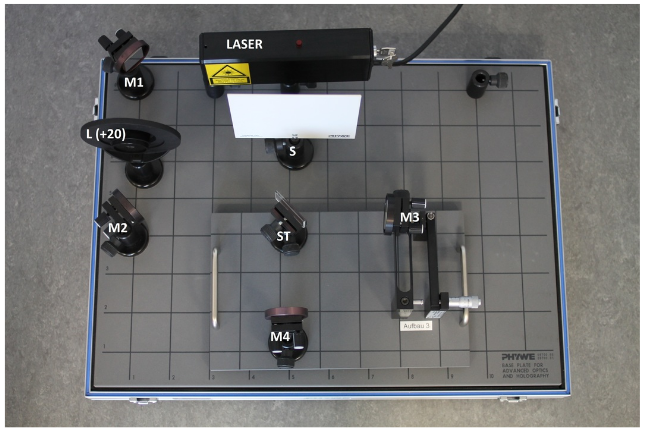
\includegraphics[width=0.7\textwidth]{Aufbau.png}
	\caption{Versuchsaufbau (Quelle: Praktikumsskript)}
	\label{Aufbau}
\end{figure}


\subsection{Versuchsdurchführung}
Mit dem Feinsteinstelltrieb an Spiegel M3 kann die optische Wegl"ange des zugeh"origen Strahlengangs variiert werden, sodass sich das Interferenzmuster am Schirm ver"andert: Pro Verschiebung des Spiegels um eine halbe Wellenl"ange entsteht ein neuer Interferenzring im Zentrum des Musters, das bei weiterer Verschiebung nach au\ss en wandert. Bei umgekehrter Drehrichtung der Mikrometerschraube verschwinden die Interferenzringe im Zentrum. Wir nehmen den Zusammenhang zwischen der optischen Weglänge $d$ und dem Skalenwert $s$ der Mikrometerschraube als linear an und bestimmen in diesem Versuch den Proportionalit"atsfaktor $k$:
\begin{equation}\label{eq:d=ks}
\Delta d=k\cdot \Delta s
\end{equation}
Zu diesem Zweck zählen wir die Anzahl an verschwindenden Interferenzringen $\Delta m$ in Abhängigkeit der Position der Mikrometerschraube $s$.
Wir beginnen bei einem Intensit"atsmaximum im Interferenzzentrum bei $s=7.00mm$, und z"ahlen durch Drehen der Mikrometerschraube 300 Ringe ab, wobei alle 10 Ringe der dazugeh"ohrige Skalenwert der Mikrometerschraube $s$ notiert wird. Die Mikrometerschraube hat eine minimale Skalenbreite von $10\mu m$.\\
Der Versuch wurde mit dem Gerät mit Nummer 2 durchgeführt.

\subsection{Versuchsauswertung}
Unsere Rohdaten sind in Tabelle \ref{table:RohdatenKalibrierung} (im Anhang) gelistet.
Gl.~\eqref{eq:d=ks} und Gl.~\eqref{eq:Grundgleichung} ergeben den Zusammenhang
\begin{equation}
\Delta m = \frac{2k}{\lambda}\Delta s,
\end{equation}
sodass wir k mit einer linearen Regression bestimmen können. Wir tragen $s$ gegen $\Delta m$ auf und sch"atzen unsere Unsicherheiten folgendermaßen ab:
\begin{align}\label{eq:Unsicherheit_Kalibrierung}
\sigma_{\Delta m}=0.1\\
\sigma_s=\frac{10\mu m}{\sqrt{12}}
\end{align}
Wir nehmen eine Unsicherheit auf $\Delta m$ an, weil sich das Interferenzmaximum durch die Dicke der Ringe nicht immer gleich einstellen lie\ss. Der Fehler auf $s$ ergibt sich durch den Skalenfehler der minimalen Skalenbreite von $10\mu m$. Dieser wurde wegen für vier Teilintervalle der Messreihe durchgeführt, Tab. \ref{table:kalib} fasst die Ergebnisse jedes solchen Bereichs zusammen:\\

\begin{table}[H]
	\centering
	\begin{tabular}{|c|c|c|}
		\hline 
		Bereich in mm&$k_1$&$k_2$  \\ 
		\hline 
		7-7.55 &$0.04823\pm3.359 \cdot 10^{-4}$ &$0.04876\pm3.418 \cdot 10^{-4}$  \\ 
		\hline 
		7.55-8.04&$0.05072\pm3.705 \cdot 10^{-4}$ &$0.04746\pm3.254 \cdot 10^{-4}$ \\ 
		\hline 
		8.04-8.53&$0.04789\pm4.056 \cdot 10^{-4}$ &$0.04894\pm4.233 \cdot 10^{-4}$ \\ 
		\hline 
		8.53-9.00&$0.04832\pm3.371 \cdot 10^{-4}$ &$0.04671\pm3.155 \cdot 10^{-4}$ \\ 
		\hline 
	\end{tabular} 
	\caption{Ergebnis der Kalibration im unterschiedlichen Bereichen}
	\label{table:kalib}
\end{table} 
\begin{comment}
	\begin{figure}[H]
		\centering
		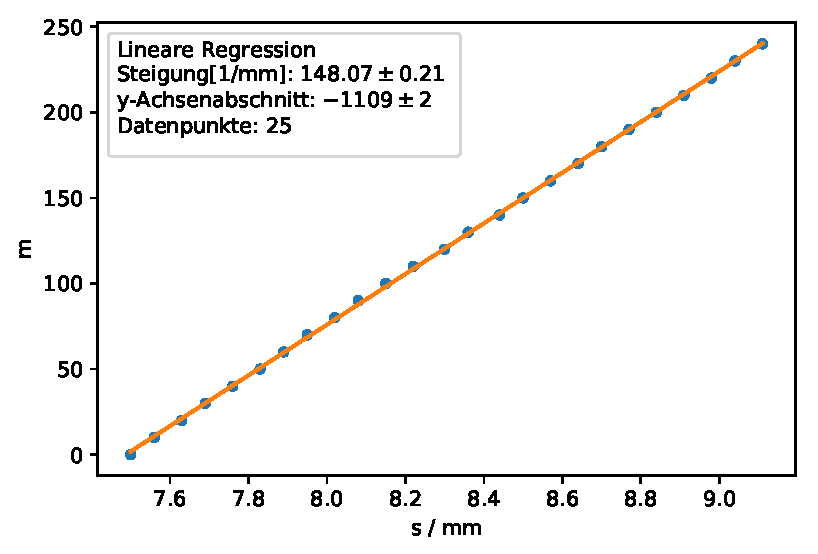
\includegraphics[width=0.6\linewidth]{Python/Uebersetzungsfaktor_LinReg.pdf}
		\caption{Lineare Regression zur Bestimmung des Kalibrierungsfaktors des Feinsteinstelltriebs: Alle Messwerte}
		\label{kLinReg}
	\end{figure}
	\begin{figure}[H]
		\centering
		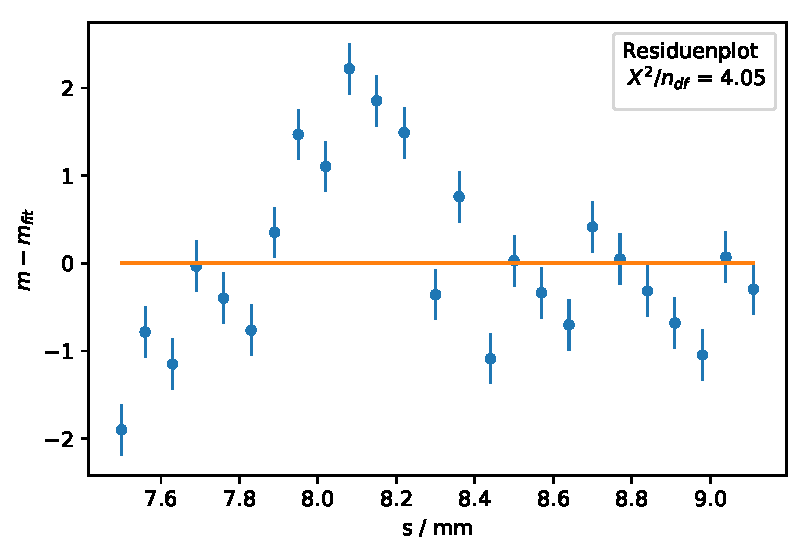
\includegraphics[width=0.6\linewidth]{Python/Uebersetzungsfaktor_Residuen.pdf}
		\caption{Residuenplot zur Bestimmung des Kalibrierungsfaktors des Feinsteinstelltriebs: Alle Messwerte}
		\label{kResPlot}
	\end{figure}
\end{comment}



\section{Bestimmung der Wellenlänge}
\subsection{Versuchsaufbau und Durchführung}
In diesem Versuch soll die Wellenlänge eines grünen Lasers mithilfe der eben bestimmten Kalibrierungskonstante $k$ des Feinsteinstelltriebs bestimmt werden. Dazu wird das Lasergerät des roten Lasers gegen das des grünen Lasers ausgetauscht. Sowohl der Versuchsaufbau als auch die Durchführung sind identisch zum vorherigen Versuch. Es werden 360 Maxima im kalibrierten Bereich der Mikrometerschraube $s\in[7.00mm,9.00mm]$ durchlaufen.
Weitere Messreihen wurden nicht in die Auswertung mit aufgenommen, weil die Messreihen entweder zu kurz sind oder sich der Experimentator bei der Abz"ahlung sehr unsicher war und deswegen zu viele Messfehler erwartet werden.
\subsection{Versuchsauswertung}
Als Erstes führen wir eine lineare Regression im gesamten Messintervall durch, um einen Eindruck über die Qualität der Daten zu erhalten. Die Ergebnisse dieses Vorgehens werden wir des Weiteren verfeinern, da wir in diesem Fall z.B. die Nichtlinearität von Gl. \ref{eq:d=ks} und die auch im Messprotokoll notierten Störungen gar nicht mitbeachten. Unsere Rohdaten sind in Tab \ref{tab:Rohdaten_gruen} und graphisch (mit der erwähnten Regression) in Abb. \ref{fig:lambdarohlinreg} zusammengefasst.
\begin{figure}[H]
	\centering
	\subfloat{{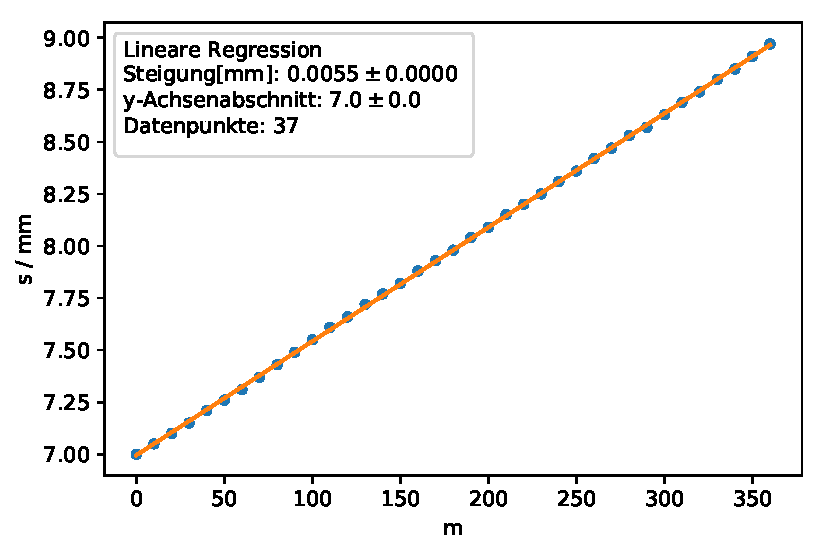
\includegraphics[width=7cm]{Python/lambda_roh_LinReg} }}
	\qquad
	\subfloat{{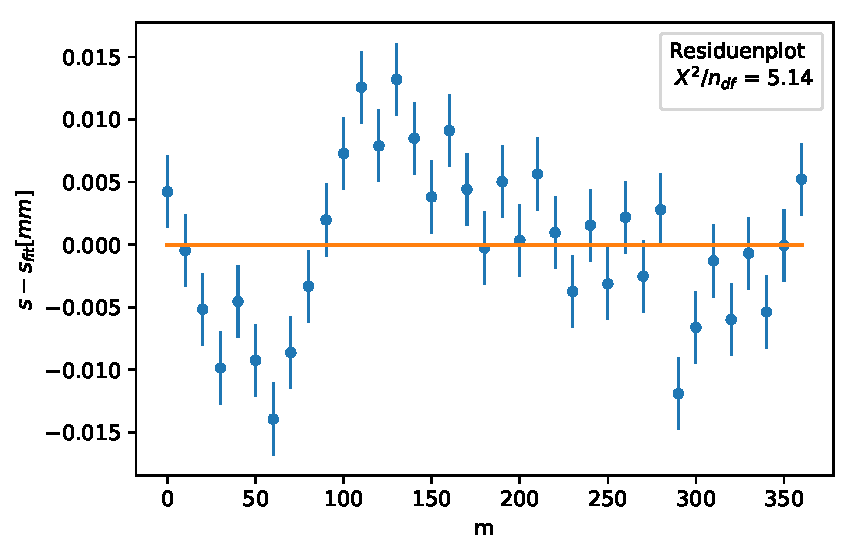
\includegraphics[width=7cm]{Python/lambda_roh_Residuen} }}
	\caption{Ergebnisse der provisorischen linearen Regression}
	\label{fig:lambdarohlinreg}
\end{figure}
Das Ergebnis der Regression beträgt
\begin{equation*}
s = (5.4694\cdot10^{-3}\pm4.5240\cdot10^{-6})mm\cdot m+(6.9958\pm9.4680*10^{-4})mm
\end{equation*}
sodass es eine grobe Wellenlänge über
\begin{equation}
	\lambda = 2a\cdot k
	\label{eq:l=2ak}
\end{equation}
von $\lambda=(523.47\pm3.2315\cdot10^{-3})$nm ergibt.\\
Im Residumplot erkennt man starke systematische Abweichungen, die wir jetzt unterdrücken möchten. Diese lassen sich unter Anderem auf Folgendes zurückzuführen: entweder hat der Experimentator die Ringe verzählt, oder das Interferenzbild wurde durch eine größere Störung verstellt, oder der Zusammenhang zwischen der Verschiebung der Spiegel und der Drehung der Schraube ist nichtlinear.\\
Um die Wellenlänge $\lambda$ genauer abschätzen zu können, teilen wir die Messreihe in vier äquidistante Intervallen auf. Für jedes einzelnes Intervall rechnen wir die Kalibrierungskonstante $k$ aus, und gehen davon aus, dass in jedem solchen Bereich die Gleichung \ref{eq:d=ks} gilt. Da zwei Messreihen für die Kalibrierung aufgenommen wurden, wird $k$ gemittelt, und die Standardabewichung der Werte als $\sigma_{k}$ genommen. Die dazugehörigen Graphen und Tabellen sind im Anhang zu finden. Ganz analog zum vorherigem Verfahren werten wir die Daten aus, die in der Abbildung \ref{fig:lambda_Intervall} zusammenfassen lassen:
\begin{figure}[H]
	\centering
	\subfloat{{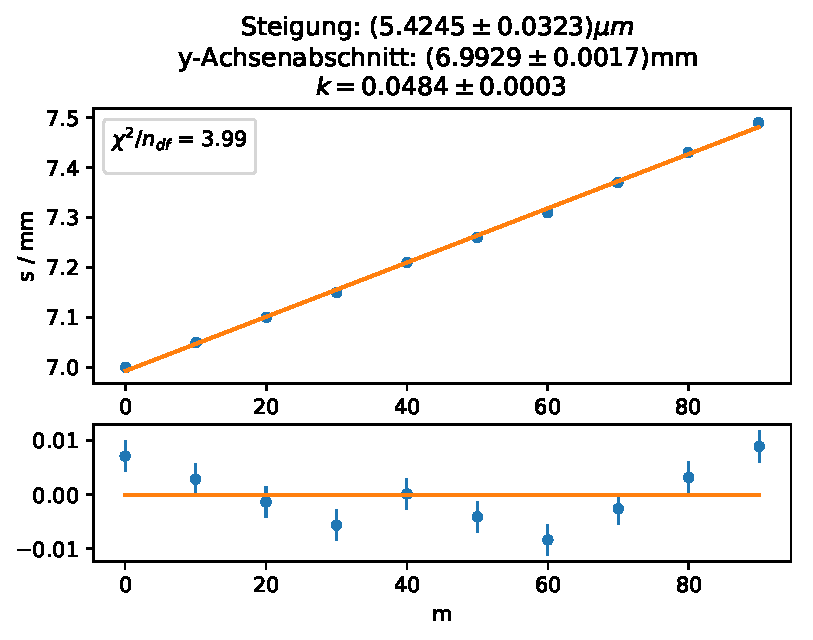
\includegraphics[width=7cm]{Python/Lambda1_mResiduen} }}
	\qquad
	\subfloat{{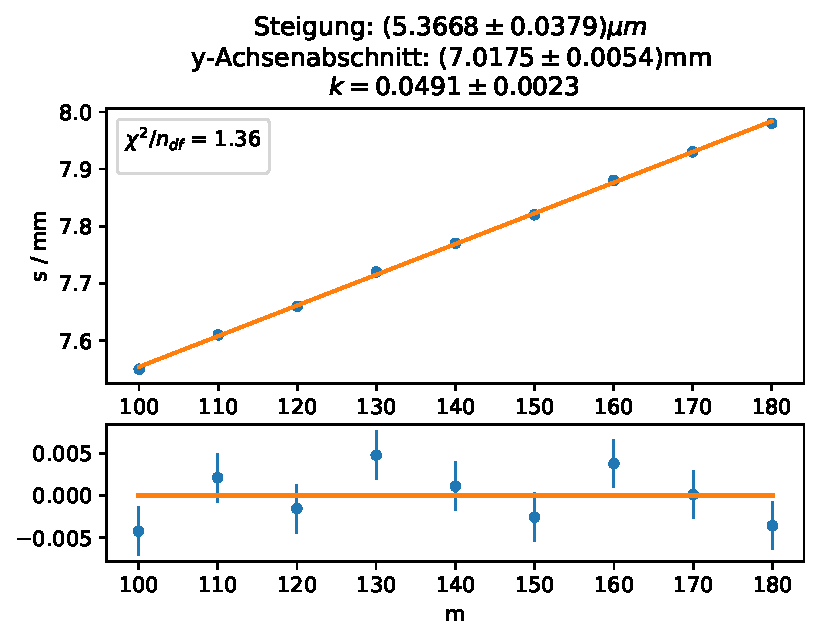
\includegraphics[width=7cm]{Python/Lambda2_mResiduen} }}
	\label{}
\end{figure}
\begin{figure}[H]
	\centering
	\subfloat{{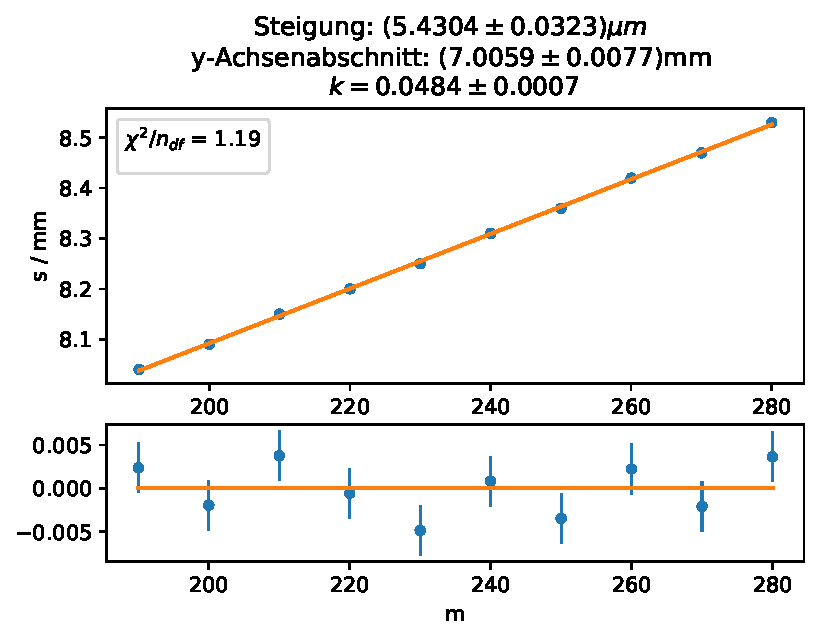
\includegraphics[width=7cm]{Python/Lambda3_mResiduen} }}
	\qquad
	\subfloat{{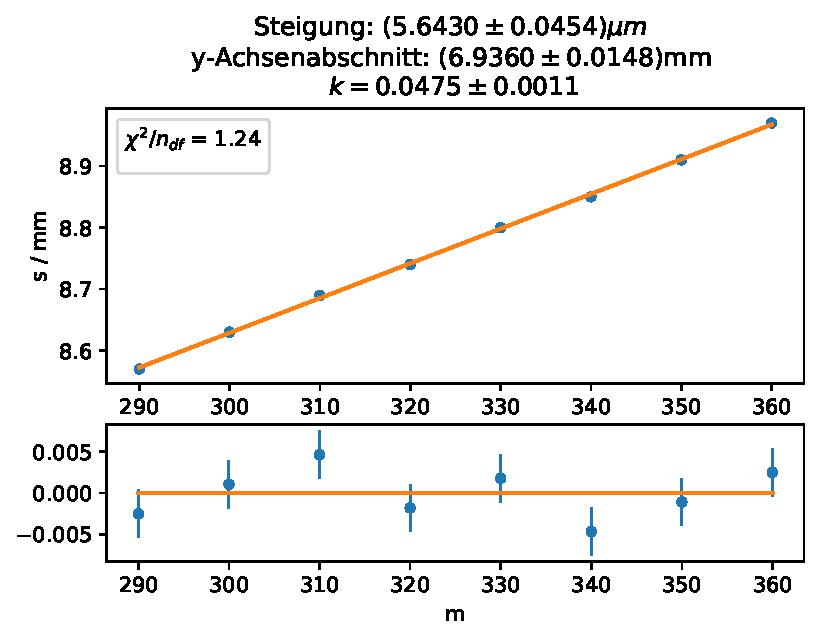
\includegraphics[width=7cm]{Python/Lambda4_mResiduen} }}
	\caption{Auswertung der Intervalle zur Bestimmung der Wellenlänge}
	\label{fig:lambda_Intervall}
\end{figure}
oder im tabellarischen Form:
\begin{center}
	\begin{tabular}{|c|c|c|c|}
		\hline 
		Bereich in mm&Bereich als m & $k$  & $a$ \\
		\hline 
		\hline 
		7-7.55&0-90& $0.0484\pm0.0003$ &$(5.424\pm0.0323)\mu m$  \\ 
		\hline 
		7.55-8.04& 100-180 & $0.0491\pm0.0023$& $(5.366\pm0.0379)\mu m$ \\ 
		\hline 
		8.04-8.53&190-280& $0.0484\pm0.0007$ & $(5.430\pm0.0323)\mu m$ \\ 
		\hline 
		8.53-9.00& 290-360 & $0.0475\pm0.0011$ & $(5.642\pm0.0454)\mu m$ \\ 
		\hline 
	\end{tabular}  
\end{center}
Aus den erhaltenen Parametern $a$ lässt sich die Wellenlänge über Gl. \ref{eq:l=2ak} bestimmen auf:
\begin{center}
	\begin{tabular}{|c|c|}
		\hline 
		Bereich in mm&$\lambda$  \\ 
		\hline 
		7-7.55&$(525.6\pm3.1(stat) \pm3.3(sys))$nm \\ 
		\hline 
		7.55-8.04&$(526.9\pm3.7(stat)\pm24.8(sys))$nm\\ 
		\hline 
		8.04-8.53&$(525.8\pm3.1(stat)\pm8.1(sys)) $nm\\ 
		\hline 
		8.53-9.00&$(536.2\pm4.3(stat)\pm12.9(sys))$nm  \\ 
		\hline 
	\end{tabular}
\end{center}
Hier stammt einmal der statistische Fehler auf $\lambda$ aus der Unsischerheit $\sigma_a$, die sich nach Gauß nach $\sigma_{\lambda} = 2k \cdot \sigma_a$ fortpflanzen lässt. Die systematische Unsicherheit wurde analog über $\sigma_k$ bestimmt, also $\sigma_{\lambda} = 2a\cdot \sigma_{k}$.\\
Man erkennt, dass selbst mit dieser Methode im ersten Bereich anhand des Residumplots immer noch eine starke Systematik erkennbar ist. Dieser liefert dementsprechend der größte $\chi^2/n_{df}$-Wert und das Ergebnis liegt im $2\sigma$-Bereich. Im zweiten und im vierten Bereich fällt es einem auf, dass die Kalibrierungsdaten (siehe Anhang) sehr unterschiedliche Werte liefern, sodass es zu einer solchen großen systematische Abweichung kommt. Des Weiteren wird also mit dem dritten Wert gerechnet, in allen der letzten drei Fällen liegt aber das Ergebnis im $1\sigma$-Bereich des erwarteten Werts.
\section{Druckabhängigkeit des Brechungsindexes von Luft}
\subsection{Versuchsaufbau und Durchführung}
Als nächstes wird die Druckabhängigkeit des Brechungsindexes von Luft untersucht. Dazu wird in den Strahlengang zwischen Strahlteiler und Spiegel M4 eine Glasparzelle (hohler Glaszylinder) der Länge $L=10mm$ befestigt. Die Glasparzelle ist über zwei Schläuche an einem digitalen Druckmessgerät und an einer Handpumpe angeschlossen. Über die Handpumpe kann der Druck in der Parzelle verringert werden, wobei der konkrete Wert des Luftdrucks am Messgerät auf 1hPa genau ausgelesen werden kann. Zunächst wird bei Normaldruck, in unserem Fall 995hPa, durch Drehen der Mikrometerschraube ein Interferenzbild erzeugt mit einem Maximum im Zentrum. Nun wird langsam der Druck in der Glasparzelle erniedrigt und bei jeder Entstehung eines neuen Interferenzrings im Zentrum der Druck notiert. Wir beenden einen Messvorgang, wenn wir einen Druck von ca. 300hPa erreichen. Insgesamt wurden 7 Messreihen durchgeführt.

\subsection{Auswertung}
Die Rohdaten der 7 Messreihen sind in Tabelle \ref{table:RohdatenDruck} aufgelistet.
\begin{table}[H]
	\centering
	\begin{tabular}{|c|c|c|c|c|c|c|c|}
		\hline
		&\multicolumn{7}{c|}{Druck $P$ der Messreihen (MR) in hPa}\\
		$\Delta m$&MR 0&MR 1&MR 2&MR 3&MR 4&MR 5&MR 6\\
		\hline
		0&992&994&994&994&994&994&994\\
		1&855&874&888&903&910&907&885\\
		2&779&762&796&811&816&811&798\\
		3&680&677&709&704&724&726&704\\
		4&582&588&596&608&620&627&598\\
		5&490&469&522&508&532&523&502\\
		6&387&381&433&414&435&430&386\\
		7&303&290&310&327&317&325&323\\
		8&&&&217&&218&\\
		\hline
	\end{tabular}
	\caption{Rohdaten Druckabh"angigkeit Brechungsindex}
	\label{table:RohdatenDruck}
\end{table}
Wir werten die Messreihen nun einzeln aus.
Der optische Weg verändert sich mit Gl.~\eqref{eq:d=nl} zu $\Delta d=2L\cdot\Delta n$. Eingesetzt in $d=m\lambda$ als Bedingung für konstruktive Interferenz ergibt sich:
\begin{align}
2L\Delta n&=\lambda\Delta m\nonumber\\
\Leftrightarrow\Delta p&=\frac{\lambda}{2L(\frac{\Delta n}{\Delta P})}\Delta m
\end{align}
Gesucht ist der Faktor $\frac{\Delta n}{\Delta P}$, um die Druckabhängigkeit des Brechungsindexes in linearer Näherung $n(P)=1+\frac{\Delta n}{\Delta P}\cdot P$ angeben zu können.\\
Im Folgenden schreiben wir $m=\Delta m$ und meinen die Anzahl an Interferenzringen, die wir ausgehen vom Normaldruck z"ahlen konnten.\\
Wir tragen für jede Messreihe $P$ gegen $m$ auf und führen eine lineare Regression durch. Dabei nehmen wir folgenden Unsicherheiten an:
\begin{align}
\sigma_{m}&=0.1\\
\sigma_{P}&=1\ hPa
\end{align}
Für den Wert von $\sigma_m$ nehmen an, dass wir die Zahl der Interferenzringe richtig abzählen, aber die genaue Position des Interferenzmaximums nicht exakt bestimmen können. Die Unsicherheit auf $P$ ergibt sich aus der Leckrate von ca. $1hPa/s$ und einer Ableseschnelligkeit von ca. $1s$. Ein Druck-Offset im Druckmessgerät ist für unsere Berechnungen irrelevant, da nur die Druckdifferenzen von Bedeutung sind. \\
Die Ergebnisse der linearen Regression sind beispielhaft anhand der Messreihen 0 und 1 in folgenden Abbildungen dargestellt.
\begin{comment}
\begin{figure}[H]
	\centering
	\begin{subfigure}{0.49\textwidth}
		\centering
		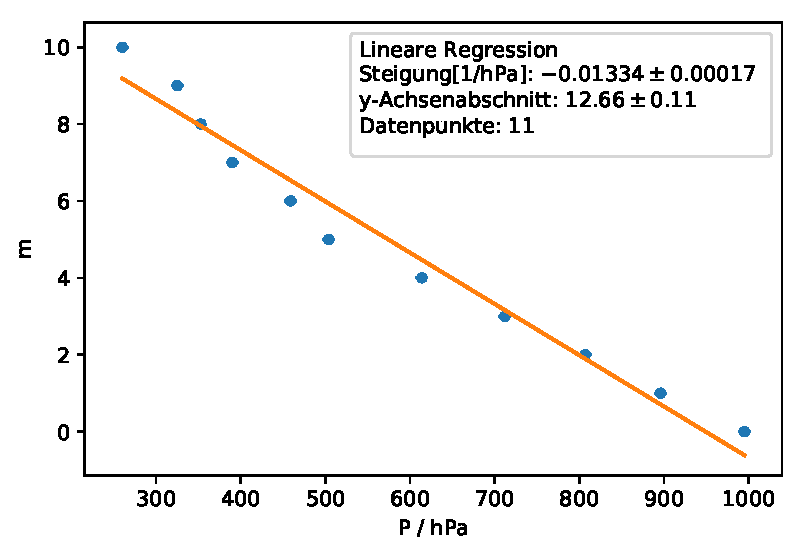
\includegraphics[width=\textwidth]{Python/MR6_LinReg_Rohdaten.pdf}
	\end{subfigure}
	\begin{subfigure}{0.49\textwidth}
		\centering
		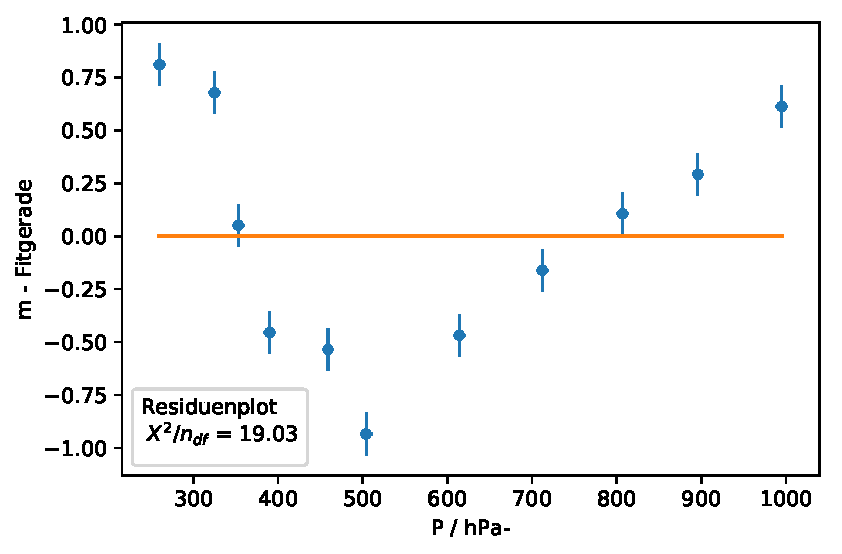
\includegraphics[width=\textwidth]{Python/MR6_Residuen_Rohdaten.pdf}
	\end{subfigure}
	\caption{Lineare Regression mit den Rohdaten der Messreihe 6}
	\label{MR6_Rohdaten}
\end{figure}
\end{comment}
Die Werte für $\chi^2/n_{df}$  der anderen Messreihen befinden sich im Bereich von 0.78 bis 1.26, sodass wir die G"ute der Fits als zufriedenstellend betrachten. Aus den Steigungen $-a$ lassen sich nun $\frac{\Delta n}{\Delta P}$ mit Unsicherheit $\sigma$ pro Messreihe bestimmen, durch
\begin{align}\label{eq:dndp_aus_Steigung}
\frac{\Delta n}{\Delta P}&=\frac{\lambda}{2La}\nonumber\\
\sigma(stat)&=\sigma_{a}\frac{\lambda}{2La^2}\nonumber\\
\sigma(sys)&=\sigma_{\lambda}\frac{1}{2La}
\end{align}
Die Ergebnisse sind in Tabelle \ref{table:Methode1_dndP} zusammengefasst und in Abb.~\eqref{Methode1_dndP} grafisch aufbereitet.
\begin{table}[H]
	\centering
	\begin{tabular}{|c|c|c|c|c|c|}
		\hline
		Messreihe&$\chi^2/n_{df}$ der&Steigung a &$\Delta n/\Delta P$&$\sigma_{\text{stat}}$&$\sigma_{\text{sys}}$\\
		&linearen Regression&[hPa]&[$10^{-7}$/hPa]&[$10^{-7}$/hPa]&[$10^{-7}$/hPa]\\
		\hline
		0&1.56&$97.0\pm1.5$&2.743&0.043&0.005\\
		1&1.35&$99.7\pm1.6$&2.667&0.042&0.005\\
		2&1.26&$95.4\pm1.5$&2.789&0.044&0.005\\
		3&0.29&$97.1\pm1.3$&2.739&0.036&0.005\\
		4&0.90&$96.2\pm1.5$&2.765&0.044&0.005\\
		5&0.78&$97.0\pm1.3$&2.742&0.036&0.005\\
		6&1.23&$97.6\pm1.5$&2.725&0.043&0.005\\
		\hline
	\end{tabular}
	\caption{Steigung und resultierendes $\Delta n/\Delta P$ pro Messreihe}
	\label{table:Methode1_dndP}
\end{table}

\begin{figure}[H]
	\centering
	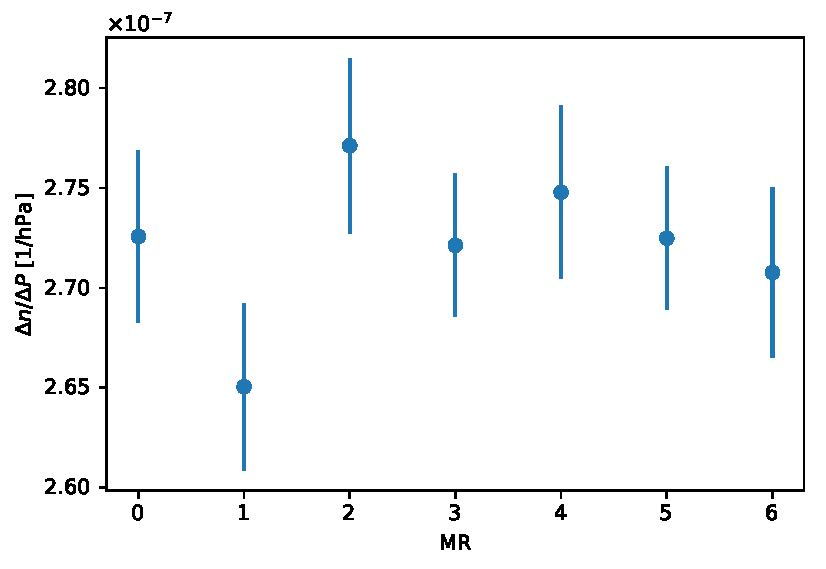
\includegraphics[width=0.6\textwidth]{Python/Methode1_Ergebnisse.pdf}
	\caption{$\Delta n/\Delta P$ für die unterschiedlichen Messreihen mit statistischem Fehler}
	\label{Methode1_dndP}
\end{figure}

Die Werte f"ur $\frac{\Delta n}{\Delta P}$ sind in ihren Unsicherheiten kompatibel. Daher berechnen wir das gewichtete Mittel aus allen Messreihen mit den statistischen Unsicherheiten.und erhalten
\begin{equation}
\frac{\Delta n}{\Delta P}=(2.713\pm 0.019(\text{stat.})\pm 0.031(\text{sys.}))\cdot10^{-7}\frac{1}{hPa}
\end{equation}
Der Literaturwert von $2.655\cdot10^{-7}\frac{1}{hPa}$ liegt in einer $1.2\sigma$-Umgebung.\\
\footnote{Würden wir mit der Herstellerangabe der Wellenlänge des grünen Festkörperlasers rechnen, w"urden wir einen Wert von $\frac{\Delta n}{\Delta P}=(2.738\pm 0.015(\text{stat.})\pm 0.005(\text{sys.}))\cdot10^{-7}\frac{1}{hPa}$ erhalten, was in einer 4$\sigma$ Umgebung des Piteraturwertes im Praktikumsskript liegt. Die Abweichung l"asst sich eventuell darauf zur"uckf"uhren, dass sich die Literaturangabe auf eine Wellenl"ange von 632nm bezieht, und sich vom Brechungsindex f"ur die Wellenl"ange im Versuch unterscheidet.}

\newpage
\section{Anhang}
\begin{table}[!htb]
	\begin{minipage}{.5\linewidth}
		\centering
		\begin{table}[H]
			\centering
			\begin{tabular}{|c|c|c|}
				\hline
				&Messreihe1&Messreihe2\\
				$\Delta m$&$s$ [mm]&$s$ [mm]\\
				\hline
				0&7.00&7.00\\
				10&7.06&7.06\\
				20&7.13&7.22\\
				30&7.19&7.17\\
				40&7.26&7.24\\
				50&7.32&7.30\\
				60&7.39&7.38\\
				70&7.46&7.46\\
				80&7.53&7.53\\
				90&7.59&7.58\\
				100&7.66&7.65\\
				110&7.71&7.71\\
				120&7.78&7.79\\
				130&7.84&7.85\\
				140&7.90&7.92\\
				150&7.97&7.99\\
				160&8.04&8.06\\
				170&8.11&8.12\\
				180&8.18&8.19\\
				190&8.25&8.26\\
				200&8.31&8.31\\
				210&8.37&8.38\\
				220&8.44&8.45\\
				230&8.51&8.51\\
				240&8.58&8.57\\
				250&8.64&8.64\\
				260&8.71&8.71\\
				270&8.77&8.78\\
				280&8.83&8.85\\
				290&8.91&8.91\\
				300&8.97&8.98\\
				\hline
			\end{tabular}
			\caption{Rohdaten Kalibrierung Feinsteinstelltrieb}
			\label{table:RohdatenKalibrierung}
		\end{table}
	\end{minipage}%
	\begin{minipage}{.5\linewidth}
		\centering
		\begin{table}[H]\centering
			\begin{tabular}{c||c}
				$\Delta m$&s [mm]\\
				\hline
				0&7.00\\
				10&7.05\\
				20&7.10\\
				30&7.15\\
				40&7.21\\
				50&7.26\\
				60&7.31\\
				70&7.37\\
				80&7.43\\
				90&7.49\\
				100&7.55\\
				110&7.61\\
				120&7.66\\
				130&7.71\\
				140&7.77\\
				150&7.82\\
				160&7.88\\
				170&7.93\\
				180&7.98\\
				190&8.04\\
				200&8.09\\
				210&8.15\\
				220&8.20\\
				230&8.25\\
				240&8.31\\
				250&8.36\\
				260&8.42\\
				270&8.47\\
				280&8.53\\
				290&8.57\\
				300&8.63\\
				310&8.69\\
				320&8.74\\
				330&8.80\\
				340&8.85\\
				350&8.91\\
				360&8.97\\
			\end{tabular}
			\caption{Rohdaten für s (grünes Licht)}
			\label{tab:Rohdaten_gruen}
		\end{table}
	\end{minipage} 
\end{table}
\newpage
\subsection{Kalibrierung - erste Messreihe}
\begin{figure}[H]
	\centering
	\subfloat{{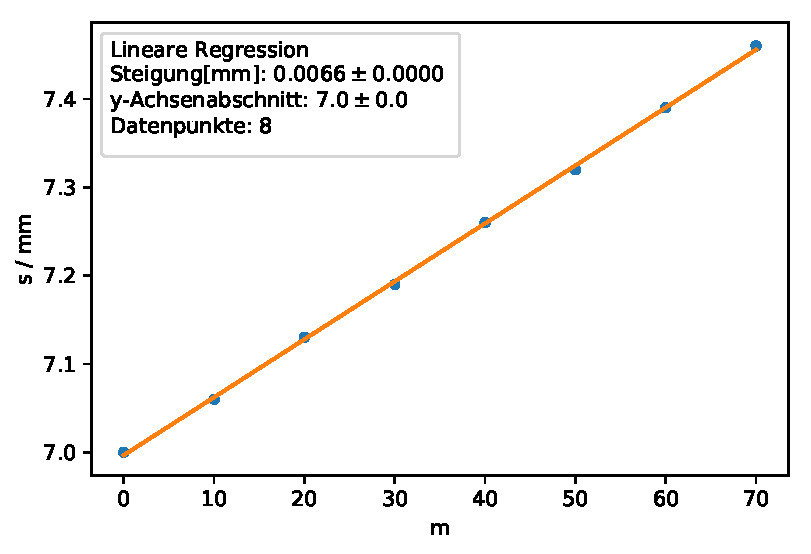
\includegraphics[width=7cm]{Python/Uebersetzungsfaktor11_LinReg}}}
	\qquad
	\subfloat{{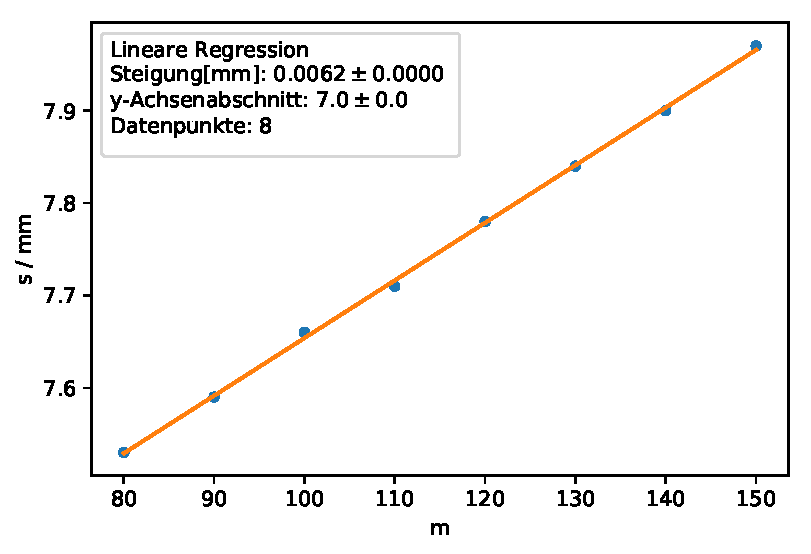
\includegraphics[width=7cm]{Python/Uebersetzungsfaktor12_LinReg} }}
	\label{}
\end{figure}
\begin{figure}[H]
	\centering
	\subfloat{{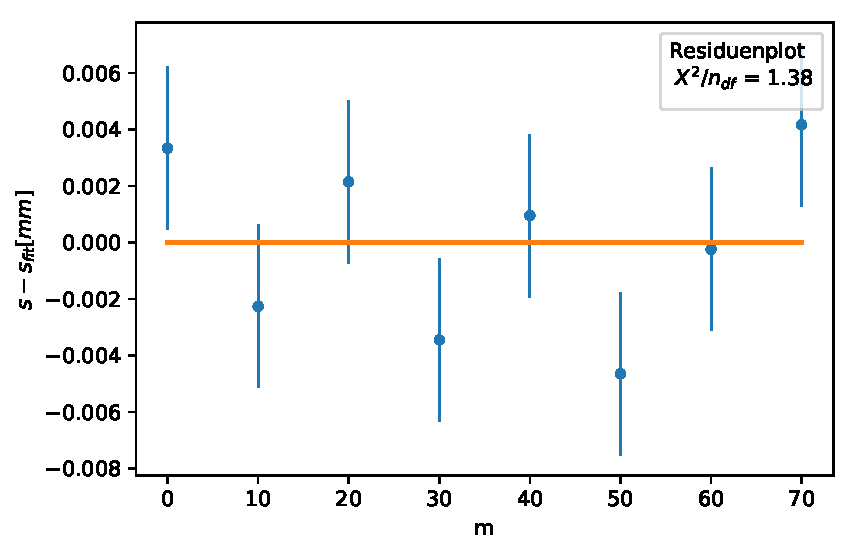
\includegraphics[width=7cm]{Python/Uebersetzungsfaktor11_Residuen} }}
	\qquad
	\subfloat{{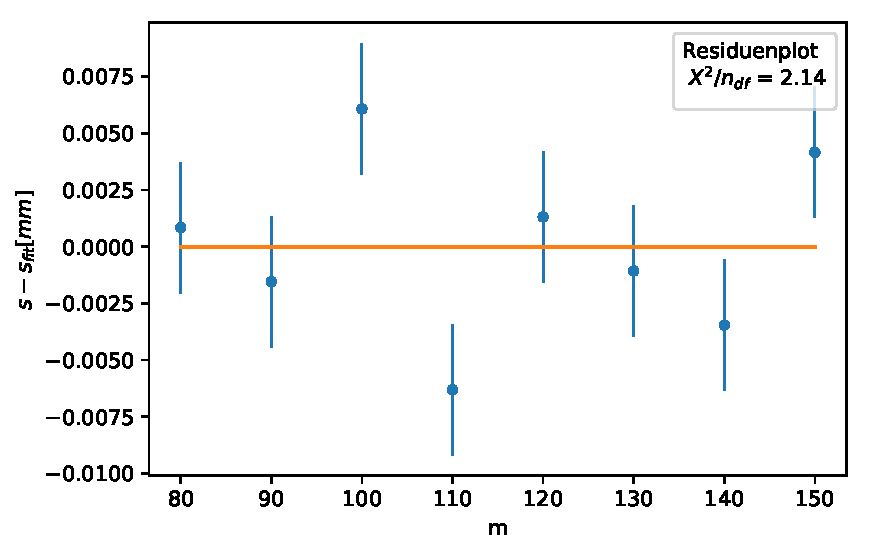
\includegraphics[width=7cm]{Python/Uebersetzungsfaktor12_Residuen}}}
\end{figure}
\begin{figure}[H]
	\centering
	\subfloat{{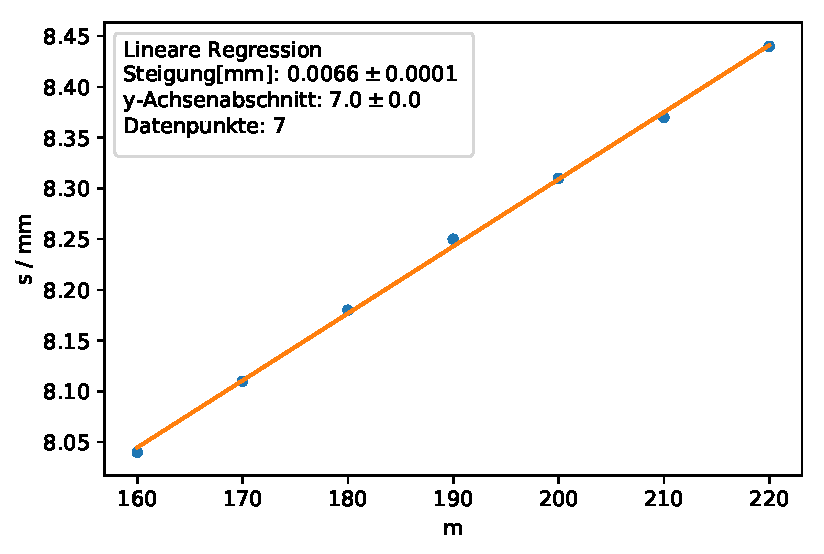
\includegraphics[width=7cm]{Python/Uebersetzungsfaktor13_LinReg}}}
	\qquad
	\subfloat{{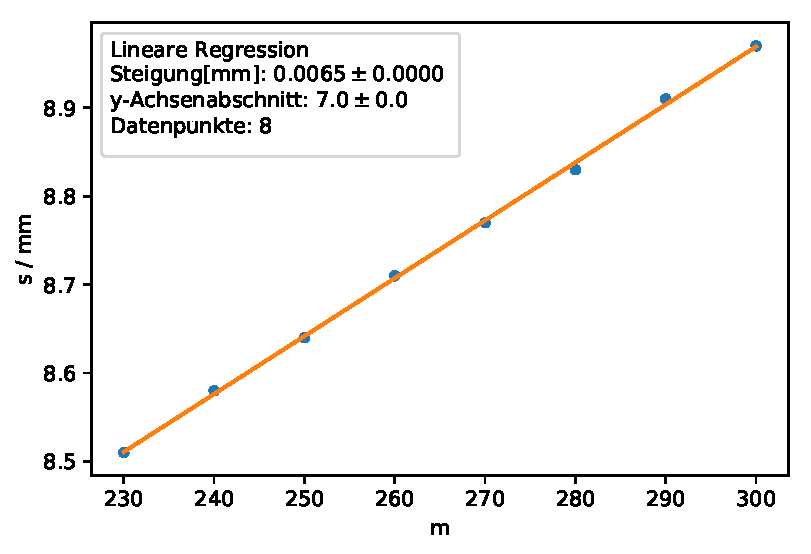
\includegraphics[width=7cm]{Python/Uebersetzungsfaktor14_LinReg} }}
	\label{}
\end{figure}
\begin{figure}[H]
	\centering
	\subfloat{{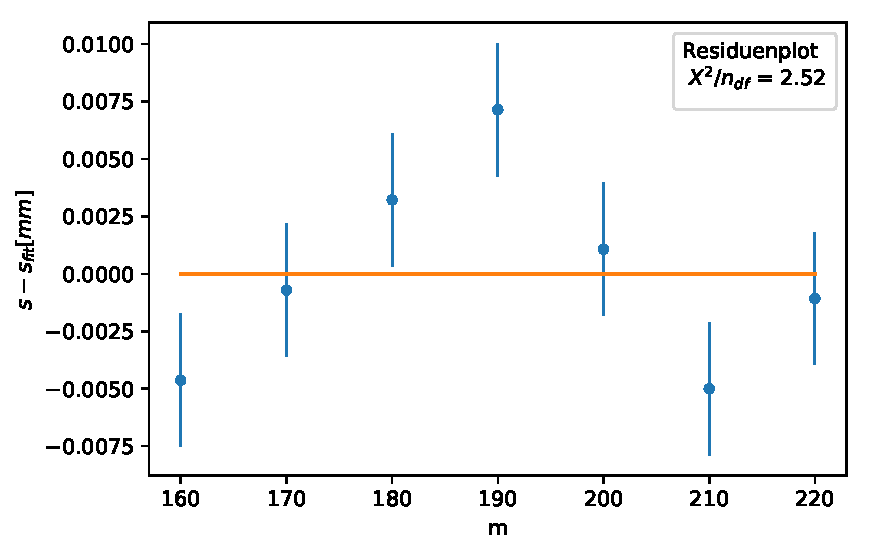
\includegraphics[width=7cm]{Python/Uebersetzungsfaktor13_Residuen} }}
	\qquad
	\subfloat{{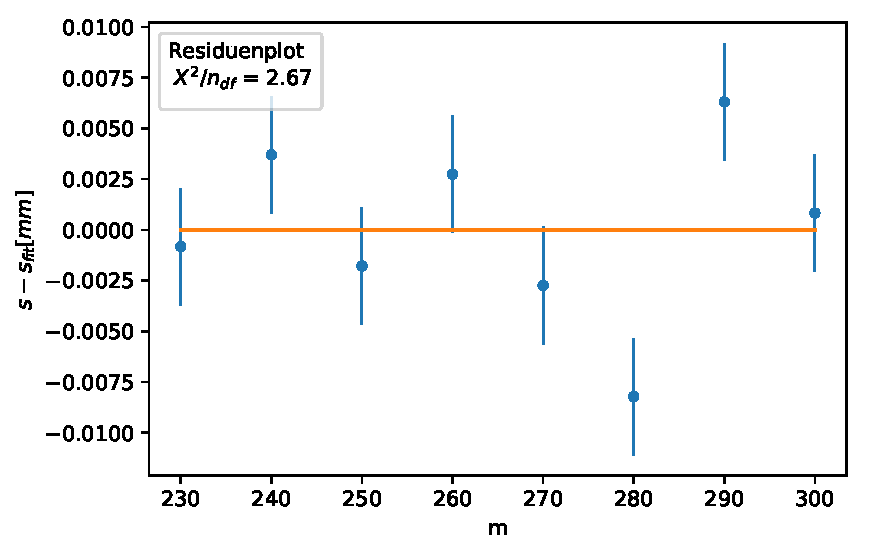
\includegraphics[width=7cm]{Python/Uebersetzungsfaktor14_Residuen}}}
\end{figure}

\subsection{Kalibrierung - zweite Messreihe}
\begin{figure}[H]
	\centering
	\subfloat{{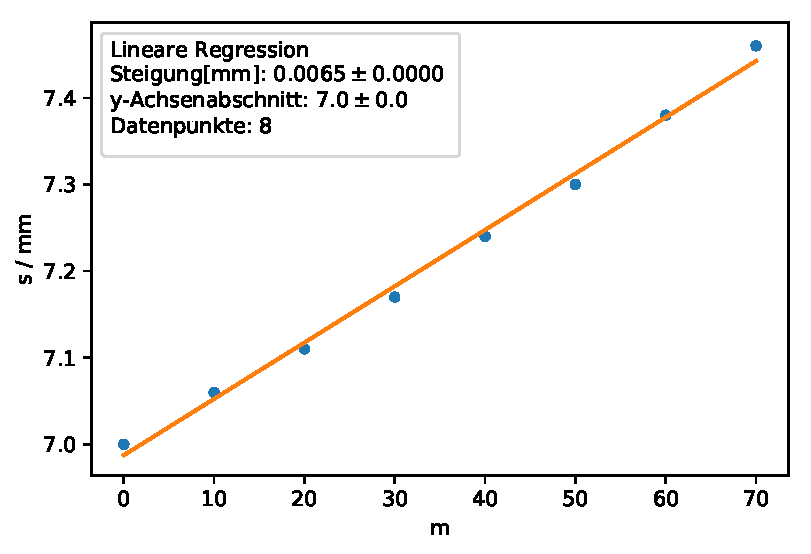
\includegraphics[width=7cm]{Python/Uebersetzungsfaktor21_LinReg}}}
	\qquad
	\subfloat{{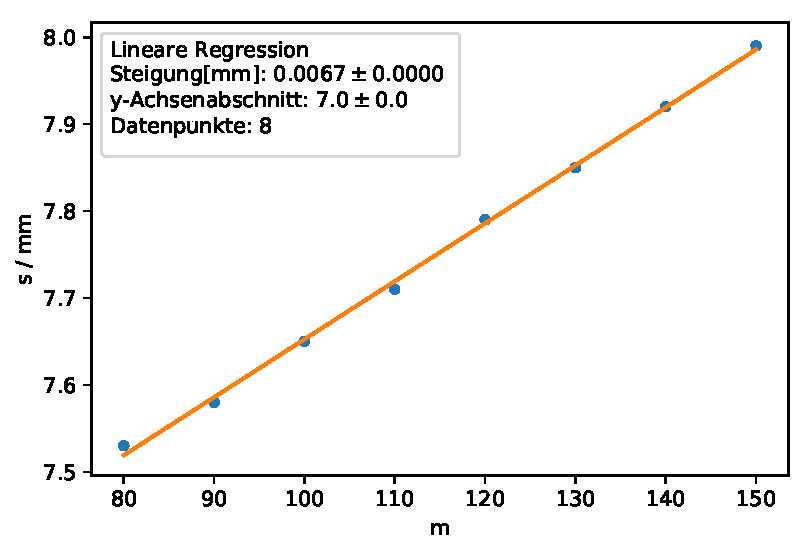
\includegraphics[width=7cm]{Python/Uebersetzungsfaktor22_LinReg} }}
	\label{}
\end{figure}
\begin{figure}[H]
	\centering
	\subfloat{{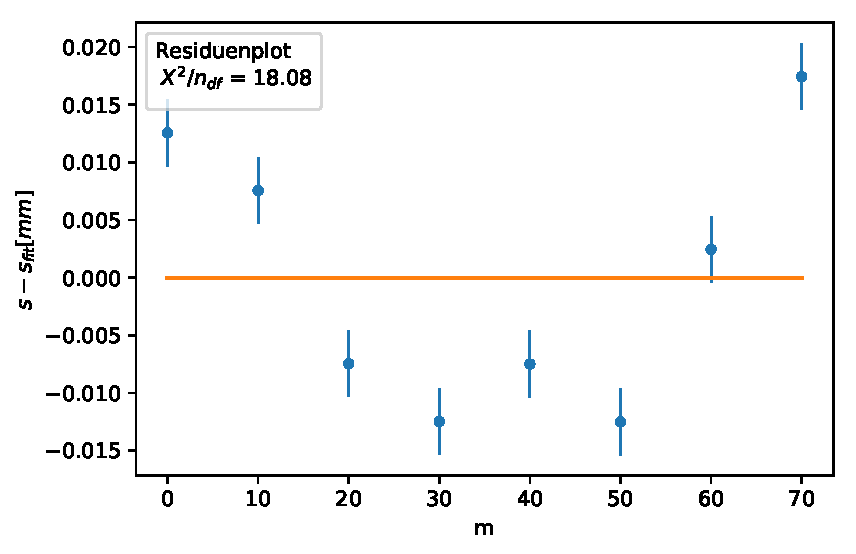
\includegraphics[width=7cm]{Python/Uebersetzungsfaktor21_Residuen} }}
	\qquad
	\subfloat{{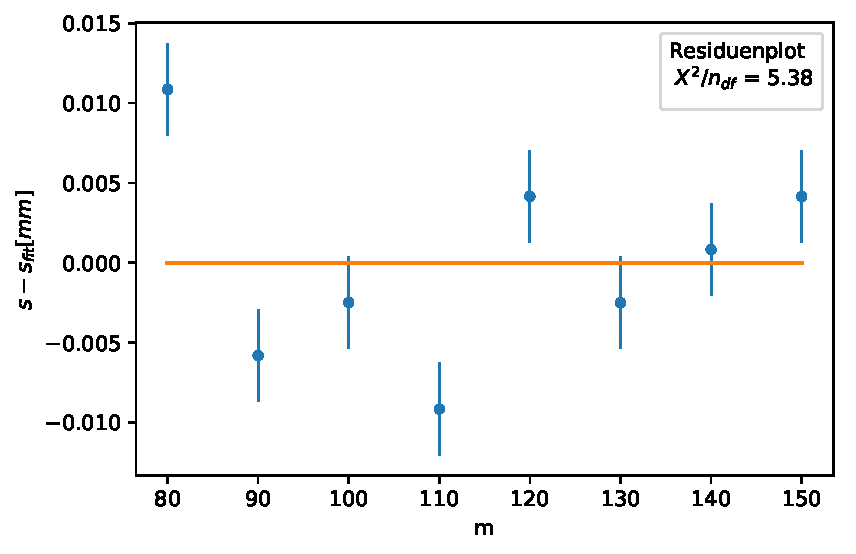
\includegraphics[width=7cm]{Python/Uebersetzungsfaktor22_Residuen}}}
\end{figure}
\begin{figure}[H]
	\centering
	\subfloat{{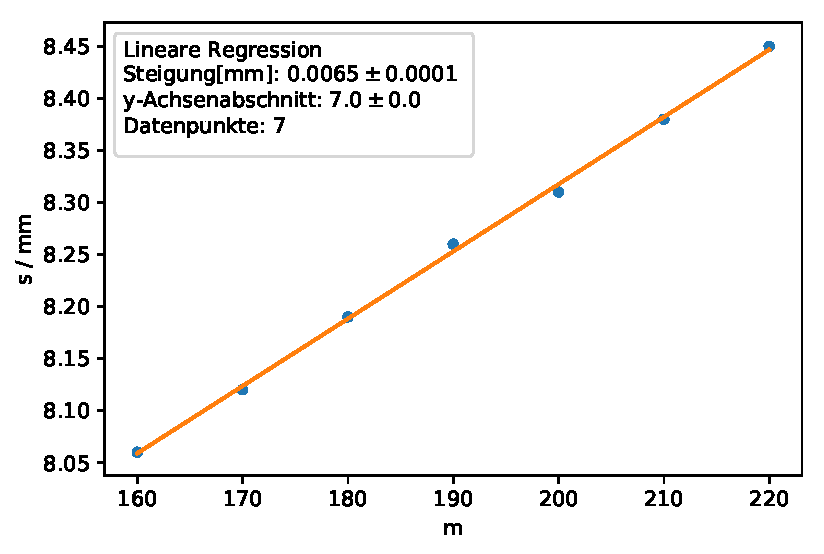
\includegraphics[width=7cm]{Python/Uebersetzungsfaktor23_LinReg}}}
	\qquad
	\subfloat{{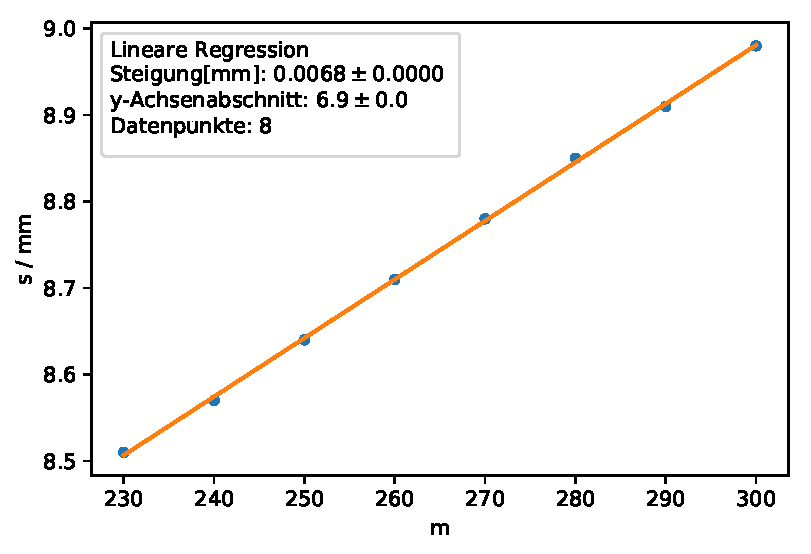
\includegraphics[width=7cm]{Python/Uebersetzungsfaktor24_LinReg} }}
	\label{}
\end{figure}
\begin{figure}[H]
	\centering
	\subfloat{{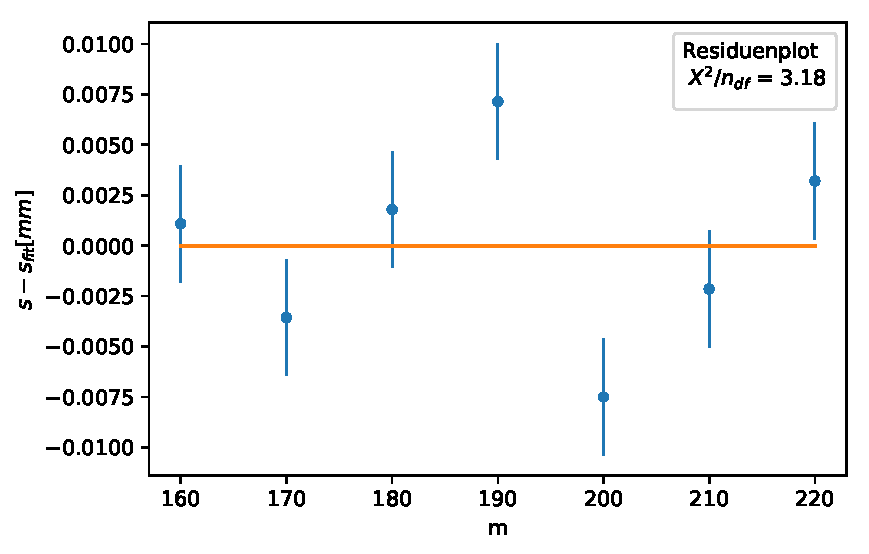
\includegraphics[width=7cm]{Python/Uebersetzungsfaktor23_Residuen} }}
	\qquad
	\subfloat{{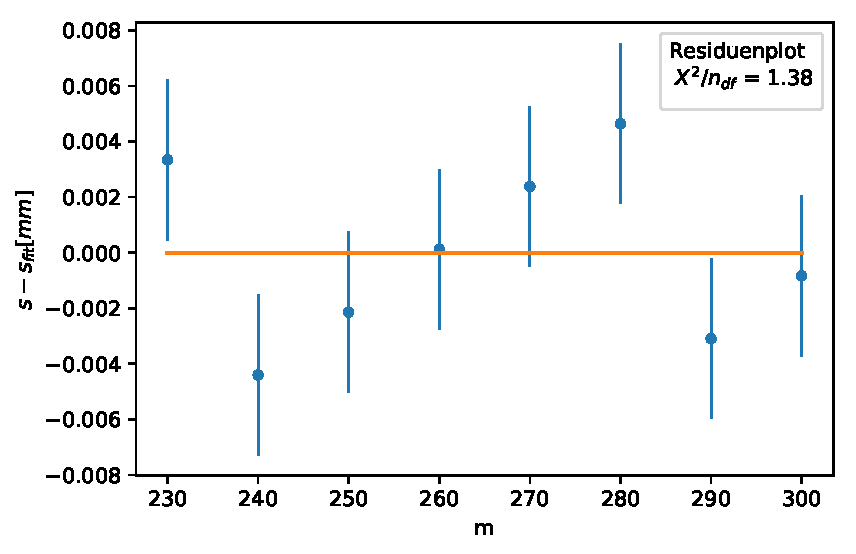
\includegraphics[width=7cm]{Python/Uebersetzungsfaktor24_Residuen}}}
\end{figure}
\end{document}